\section{Principes de DICOM}

	\frame
	{
		\frametitle{Objectifs}
		\begin{itemize}
			\item Trouver un langage commun pour l'\'echange de donn\'ees entre \'equipements d'imagerie.
			\item Pousser les vendeurs \`a communiquer avec ce langage commun.
			\item Standardiser :
			\begin{itemize}
				\item le stockage (i.e. format de fichier) ;
				\item et la communication des donn\'es (i.e. protocoles de communication).
			\end{itemize}
			\item Offrir les services de base \`a toute nouvelle connexion, sans changement d'un quelconque composant logiciel (\emph{i.e.~Plug~\&~Play}) :
    			\begin{itemize}
        				\item interrogation du PACS, d'une worklist ;
        				\item r\'ecup\'eration / affichage d'images d'autres fournisseurs ;
        				\item production d'images lisibles par tout syst\`eme respectant la norme.
        			\end{itemize}
		\end{itemize}
	}

	\frame
	{
		\frametitle{Prescription d'un examen radiologique}
		\begin{itemize}
			\item Sch\'ematisation de la proc\'edure :
			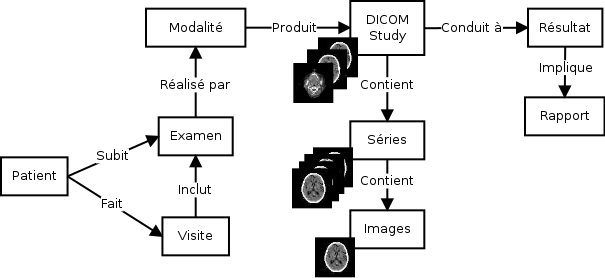
\includegraphics[width=\linewidth]{./figures/scenario.png}
			\item Donn\'ees et relations d\'ecrites par la norme DICOM.
			\item Pr\'ecision du contenu et des liens d\'ependante des outils et des utilisateurs (\emph{e.g.} RIS, PACS).
		\end{itemize}
	}

	\frame
	{
		\frametitle{Traduire le r\'eel en num\'erique}
		
		\begin{itemize}
			\item Un objet DICOM combine :
			\begin{itemize}
				\item des donn\'ees, ou informations (e.g. un patient, une image, \ldots)
				\begin{itemize}
					\item contenues dans un \emph{Information Object},
					\item d\'efini dans la norme par une \emph{Information Object Definition} (ou \emph{IOD}) ;
				\end{itemize}
				
				\item et une fonction pr\'ecise (e.g. stocker, imprimer,\ldots)
				\begin{itemize}
					\item c'est-\`a-dire un \emph{Service},
					\item d\'efini par un \emph{DICOM Message Service Element} (ou \emph{DIMSE})
				\end{itemize}
			\end{itemize}
			\item Une norme doit lister toutes les combinaisons possibles.
		\end{itemize}
	}
	
	\frame
	{
		\frametitle{Un identifiant unique : le SOP Class UID}

		\begin{itemize}
			\item La combinaison Information Object + Service est :
			\begin{itemize}
				\item appel\'ee \emph{Service/Object Pair} (ou \emph{SOP}) ;
				\item un \'el\'ement important pour d\'eterminer la conformit\'e \`a la norme ;
				\item identifi\'ee par un identifiant unique nomm\'e \emph{SOP Class UID}.
			\end{itemize}
			
			\item Norme DICOM = annuaire de SOP.\\
			SOP Class UID (identifiant unique d'un type de paire service/objet) = num\'ero unique pour trouver \`a quelle paire Service/Objet correspond un objet.
			\item Analogie : annuaire invers\'e\\
			Un num\' ero = paire \{nom $+$ adresse\}.
			\item Exemples de SOP Class UID :
			\begin{description}
				\item[$1.2.840.10008.5.1.4.1.1.1$] CR Image Store (enregistrer un CR) ;
				\item[$1.2.840.10008.5.1.4.1.1.2$] CT Image Store (enregistrer un CT).
			\end{description}
		\end{itemize}
	}
	
	\frame
	{
		\frametitle{Sch\'ema de construction du SOP}
		\begin{center}
			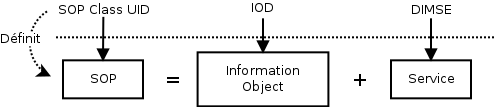
\includegraphics[width=\linewidth]{./figures/sop-definition.png}
		\end{center}		
	}

